\section{Introduction}
\label{sec:intro}
\comments{
    C-RAN is the future in 5G.
    The functions of base station (eNB) are splitted into remote radio head (RRH) and Baseband Unit (BBU).
    It is preffered to be implemented in a centralized and virtualized manner.
}

\comments{
    \textbf{Motivations.} 
    a) virtualization of C-RAN on general-purpose processors (GPPs) together with MEC is better than no virtualization, which benefits from energy saving, and network simplicity \cite{cran-survey};
    b) jointly dynamic computation resource allocation for BBU and MEC;
}

In this paper, we propose a novel framework where both BBU tasks and general edge computing tasks are processed simultaneously in a homogeneous edge cloud with general-purposed processors.
Our major contributions in this new optimization scenario are summarized as follows.
\begin{itemize}
    \item We propose a joint computation resource allocation scheme under MDP framework;
    \item We propose the parameterized computation model for BBU functions on general purpose processor, and carry out experiments to examine the parameter fitness;
    \item The performance bound of our proposed algorithm is proved.
\end{itemize}

\begin{figure*}[htb!]
    \centering
    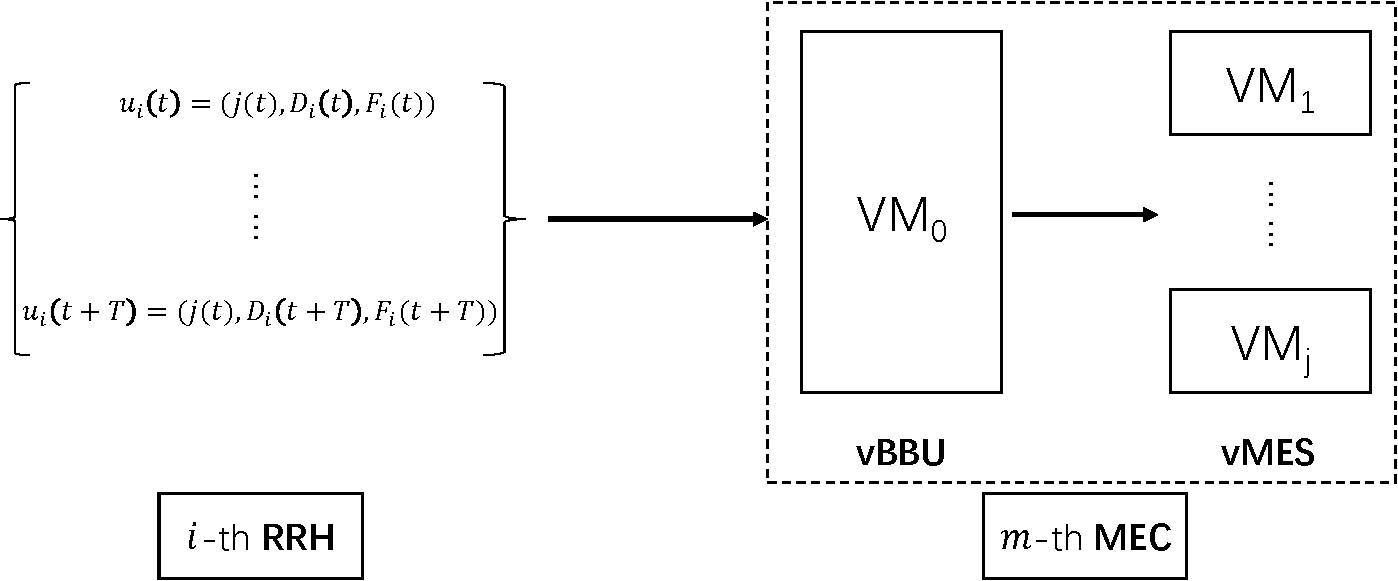
\includegraphics[width=0.9\textwidth]{images/cran-system-model.pdf}
    \caption{The Illustration of System Model.}
    \label{fig:system-model}
\end{figure*}